\chapter{Same-sign dilepton final state}
\mytodo{make todo}

\section{Contributions to \tttt production}

\subsection{On-shell}
\mytodo{2hdm, dark matter}

\subsection{Off-shell}

\subsubsection{Top quark yukawa coupling}

The SM $pp \rightarrow \tttt$ process includes diagrams with virtual Higgs bosons,
as shown in Fig.~\ref{fig:feynYukawa}. 
The amplitude corresponding to these diagrams is 
proportional to the square of the top Yukawa coupling,
and thus, the cross section of SM \tttt provides
a promising probe into the top Yukawa coupling.

\begin{figure}[!hbtp]
\centering
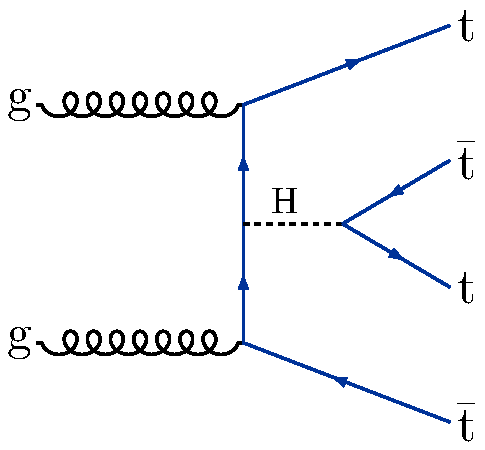
\includegraphics[width=.35\textwidth]{figs/ftp/ftdiag3.pdf} \\
\caption{One of the Feynman diagrams for \tttt including a virtual Higgs.}
\label{fig:feynYukawa}
\end{figure}

Using the notation of Reference~\cite{THEORY:TopYukawaTTTT} the \tttt cross section can be written 
as 

\begin{equation} 
\label{eq:yukawa}
\sigma(\tttt) = \sigma^{\text{SM}}(\tttt)_{g+Z/\gamma} + k_t^4 \sigma^{\text{SM}}(\tttt)_H + k_t^2 \sigma^{\text{SM}}_{\rm int}
\end{equation} 

\noindent where $k_t \equiv y_t/y_t^{\text{SM}}$, $y_t$ is the top Yukawa coupling, and $y_t^{\text{SM}}$ is its SM value.
In equation~\ref{eq:yukawa} the first term on the right hand side corresponds to the 
SM contribution to the cross section from diagrams with gluons or $Z/\gamma$, the second term
is the contribution from diagrams with virtual Higgs bosons, and the third term is the interference between
the two previous terms. Therefore, given a theoretical calculation and a measurement of $\sigma(\tttt)$, one can put 
constraints on $|y_t/y_t^{\text{SM}}|$.

The authors of Reference~\cite{THEORY:TopYukawaTTTT} have calculated the cross section terms at LO.
These are given in Table~\ref{tab:yukawa} and are shown in Fig.~\ref{fig:cross_section_yt},
where the figure shows a curve normalized such that the prediction matches the NLO calculation of 
the \tttt cross section of $12.0^{+2.2}_{-2.5}\unit{fb}$ calculated in Ref.~\cite{THEORY:Frederix2017wme}.

\begin{table} [h!]
\begin{center}
\begin{tabular}{l|c}
\hline
   & [lower, central, upper] \\
\hline
$ \sigma^{\text{SM}}(\tttt)_{g+Z/\gamma}  $ & [14.104, 9.997, 6.378] fb \\
$ \sigma^{\text{SM}}(\tttt)_H $                  & [1.625, 1.167, 0.7655] fb \\
$\sigma^{\text{SM}}_{\rm int} $                   & [-2.152, -1.547, -0.999] fb \\
\hline
\end{tabular}
\caption{LO calculation of the terms in equation~\ref{eq:yukawa} from
Reference~\cite{THEORY:TopYukawaTTTT}.  
The uncertainties are from private communications with the authors.}
\label{tab:yukawa}
\end{center}
\end{table}


\begin{figure}[!htbp]
    \centering
    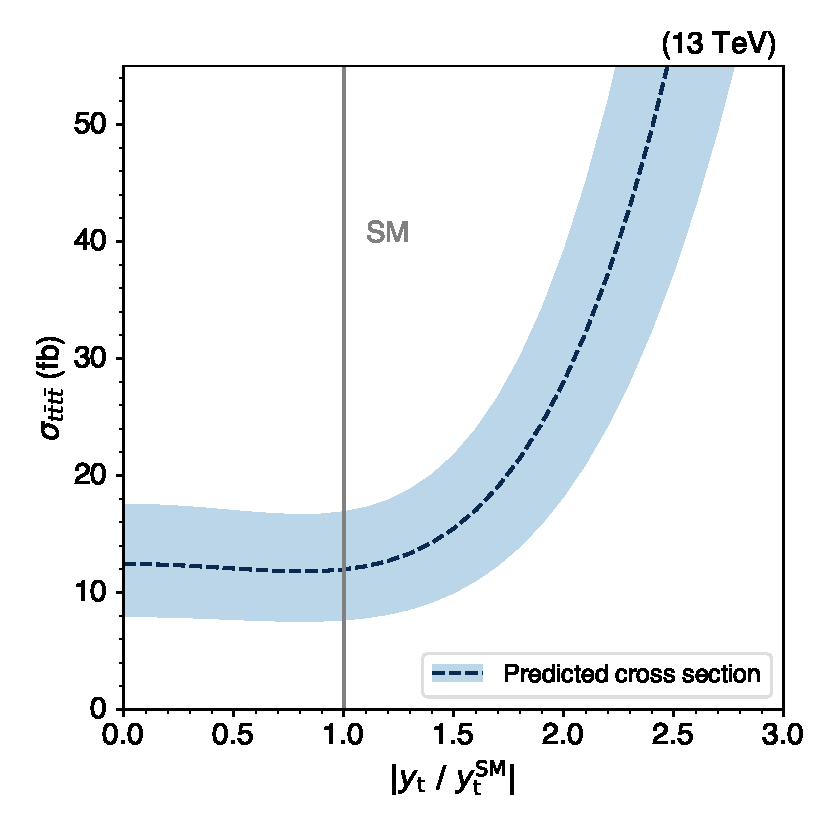
\includegraphics[width=0.75\linewidth]{figs/ftan/cross_section_yt.pdf}
    \caption{
        Predicted \tttt cross section as a function of $|y_t/y_t^{\text{SM}}|$.
    }
    \label{fig:cross_section_yt}
\end{figure}

\subsubsection{Light off-shell mediators}

The production of \tttt may also be influenced by a neutral scalar mediator
($\phi$) or neutral vector mediator ($Z'$) which couple to top quarks and have
masses less than twice the mass of the top quark, distinguishing them from
from similar processes within the 2HDM framework, for example. The off-shell contributions
to the SM \tttt production can be large, as shown in
Ref.~\cite{THEORY:Alvarez2016nrz}. For a large range of masses, the authors have
shown that kinematics are identical when considering these additional
processes, so that the total \tttt cross section is subject to a simple
rescaling.  Corresponding coupling terms in the lagrangian of the form
\begin{equation}
    \mathcal{L}_{Z'}=-g_{t Z'}\bar{t}_R \slashed{Z}' t_R
    \quad\quad\quad
    \mathcal{L}_{\phi}=-g_{t \phi}\bar{t}_L \phi t_R
\end{equation}
There is an approximate independence of kinematics on the coupling strength and mediator mass,
so a single upper limit on the \tttt cross section can be used to place constraints 
on couplings $g_{tZ'}$ and $g_{t\phi}$ as a function of masses $m_{Z'}$ and $m_{\phi}$,
respectively.
Cross sections of \tttt (normalized to SM) as a function of $g_{tZ'}$ 
and $g_{t\phi}$, for different assumptions of $m_{Z'}$ and $m_{\phi}$,
are shown in Fig.~\ref{fig:cross_section_zprimephi}. To illustrate a particular example,
the horizontal dotted line in the figures represents excluding cross sections more than
double that of the SM. These are translated into exclusions on $g_{tZ'}$ and $g_{t\phi}$
via crossing points that are projected onto the x axis.

\begin{figure}[!htbp]
    \centering
    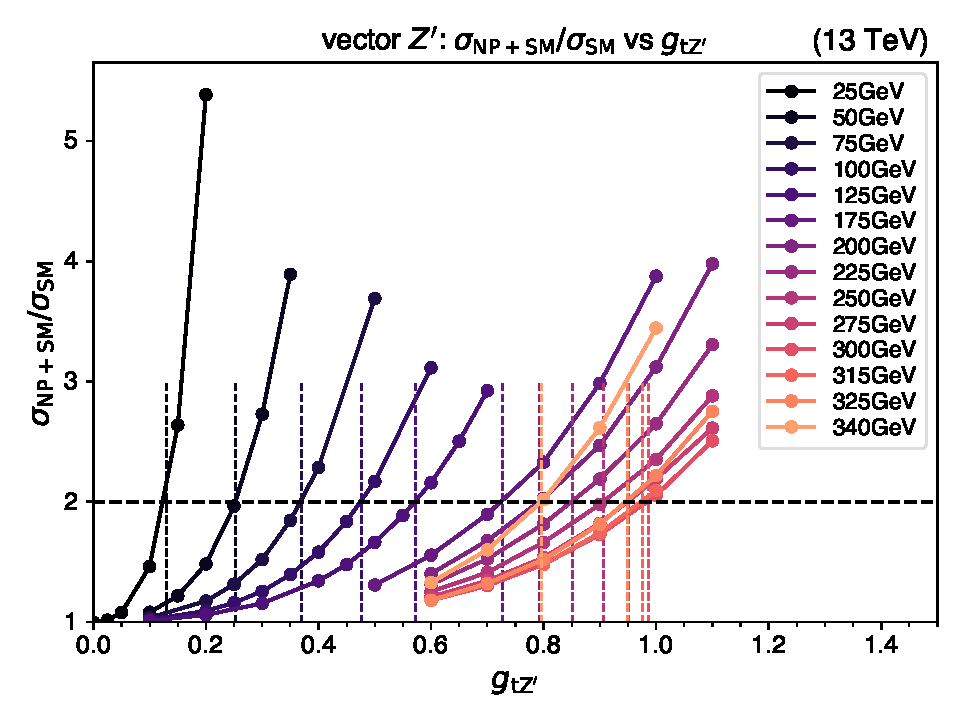
\includegraphics[width=0.78\linewidth]{figs/ftan/plot_xsec_zprime.pdf} \\
    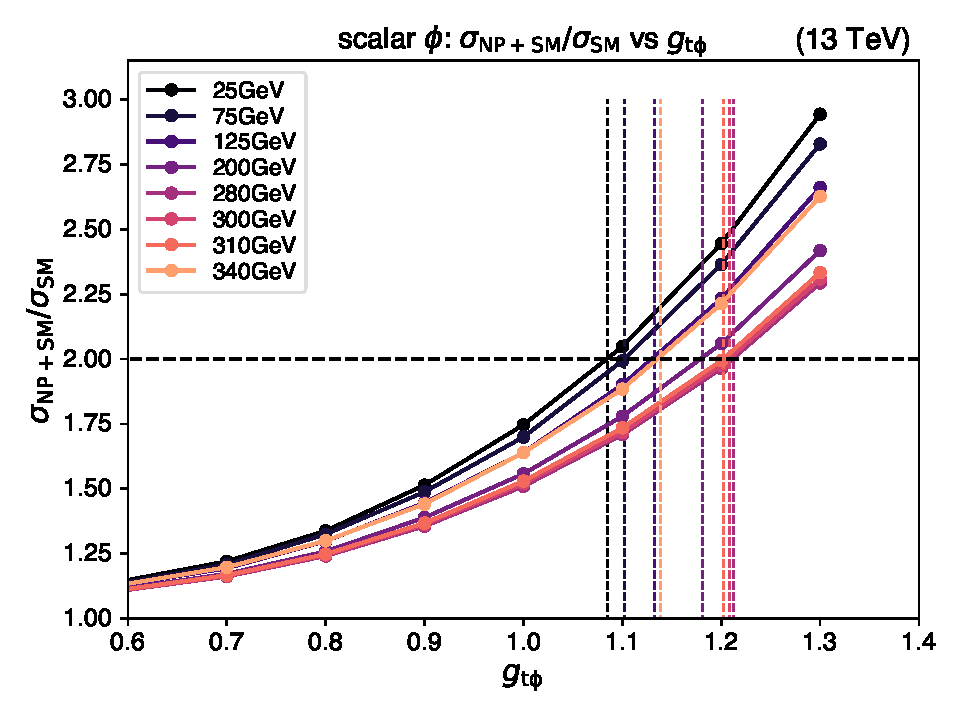
\includegraphics[width=0.78\linewidth]{figs/ftan/plot_xsec_phi.pdf}
    \caption{
        Cross sections of \tttt (normalized to SM) as a function of $g_{tZ'}$ (upper)
        and $g_{t\phi}$ (lower) for different assumptions of $m_{Z'}$ and $m_{\phi}$,
        respectively.
    }
    \label{fig:cross_section_zprimephi}
\end{figure}

\subsubsection{Oblique Higgs parameter}

In a universal effective field theory framework, the Higgs oblique
parameter $\hat H$, defined as the Wilson coefficient of the dimension-6
operator modifying the Higgs boson propagator, can result in deviations of the
SM \tttt cross section, as shown in Ref.~\cite{THEORY:ObliqueHiggs2019}.  These
(off-shell) deviations can be constrained to a level which is competitive with
constraints from on-shell processes.

The two main characteristic effects of this oblique parameter are
an additional term in the SM Higgs boson propagator
\begin{equation}
    P_h(p^2)\approx\frac{i}{p^2-m_h^2}-\frac{i\hat{H}}{m_h^2},
\end{equation}
and a rescaling of the fermionic higgs
couplings
\begin{equation}
    \kappa_f = 1-{\hat H}.
\end{equation}

Using the latest combined fits of ATLAS for the (on-shell) fermionic couplings,
with 80$\mathrm{fb}^{-1}$ of 13TeV data, the authors of Ref.~\cite{THEORY:ObliqueHiggs2019} find a constraint on
the oblique parameter of $\hat{H} < 0.16$ at 95\% CL.

The authors also calculate that the cross section of (off-shell) \tttt is subject to a fractional modification (with respect to the SM cross section)
at 14 TeV, given by,
\begin{equation}
    \frac{\sigma_{\hat{H}+\mathrm{SM}}}{\sigma_\mathrm{SM}} = 1 + 0.03\left(\frac{\hat{H}}{0.04}\right) + 0.15\left(\frac{\hat{H}}{0.04}\right)^2.
\end{equation}
For an oblique parameter value of 0.1, the formula predicts a doubling of the SM cross section of \tttt.

The SM model within the MadGraph~\cite{THEORY:MADGRAPH5} generator was modified to take into account the extra term in the propagator, as
well as the rescaling of the top-yukawa coupling, and the calculation is repeated
at 13\TeV. The resulting curve is shown in Fig.~\ref{fig:higgs_oblique_madgraph}.

When searching for SM \tttt and placing upper limits on the production cross
section, one can use the relative size of the upper limit with respect to
the SM prediction to exclude $\hat{H}$ values above a threshold. For example,
excluding cross sections more than double that of the SM, $\hat{H}$ values
above approximately 0.14 can be excluded. There are two important caveats
that will need to be taken into account when performing an interpretation for
$\hat{H}$. First, the kinematics of $\tttt$ will be slightly different
depending on the value of $\hat{H}$. Second, the SM process $\ttH$, which is
relevant for the $\tttt$ search, is proportional to
$y_\mathrm{t}^2=(1-\hat{H})^2$ ($\approx 0.74$ at $\hat{H}=0.14$).

\begin{figure}[!htbp]
    \centering
    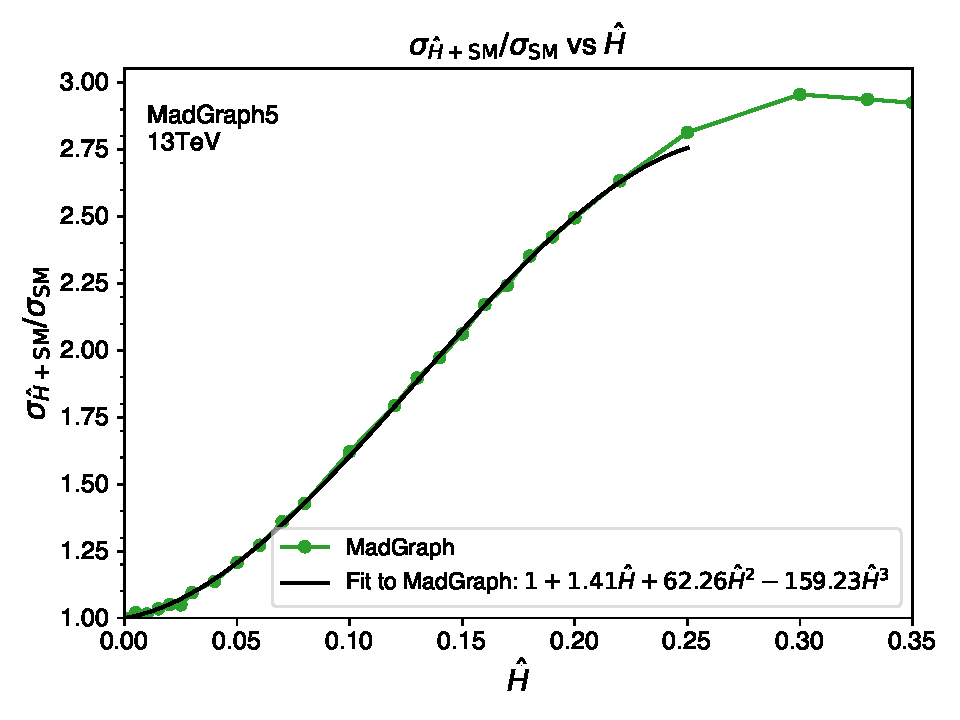
\includegraphics[width=0.75\linewidth]{figs/ftan/higgs_oblique.pdf}
    \caption{
        Cross section (normalized to SM) as a function of oblique parameter $\hat{H}$.
        The green curve is a calculation from MadGraph at 13TeV, and
        the solid black curve is a cubic fit to the calculation.
    }
    \label{fig:higgs_oblique_madgraph}
\end{figure}